\documentclass[12pt,fleqn]{article}\usepackage{../common}
\begin{document}
Orneklem Dagilimlari (Sampling Distributions)

$\frac{\bar{Y}-\mu}{\sigma / \sqrt{n}}$ ve $\frac{\bar{Y}-\mu}{S /
  \sqrt{n}}$ Karsilastirmasi

Diyelim ki normal olarak dagildigini bildigimiz bir nufustan $Y_1,..,Y_n$
rasgele orneklemini topladik, ve amacimiz bilinmeyen gercek $\mu$ hakkinda
bazi sonuclara varmak. Eger varyans $\sigma^2$ biliniyorsa, bu noktadan
sonra ne yapacagimiz gayet acik: daha once gordugumuz gibi bir karar kurali
ortaya cikartmak, ya da guven araligi hesaplamak cok kolay, ki bu
tekniklerin temelinde $Z = \frac{\bar{Y}-\mu}{\sigma / \sqrt{n}}$ dagiliminin standart normal $f_Z(z)$'ye 
yaklasmasi yatiyor. 

Fakat pratikte $\sigma^2$ genellikle bilinmez, o zaman nufus varyansinin
tahmin edicisi $S^2 = \frac{1}{n-1}\sum_{i=1}^n (Y_i-\bar{Y})^2$
kullanilir, ki bu maksimum olurluk tahmin edicisinin yansiz (unbiased)
versiyonu. Fakat buradaki onemli soru su: $\sigma^2$ yerine $S^2$ koyma Z
oranini nasil etkiler? Daha once buyuk orneklemler icin bir fark
olmadigindan bahsettik. Peki kucuk orneklemler icin? 

Kucuk $n$ icin bu iki oraninin birbirinden farkli oldugununun kesfi William
Sealy Gossett adli arastirmaciya ait. 1899'da Oxford'dan Kimya ve Matematik
bolumunden mezun olduktan sonra Gossey, Guiness adli sirkette calismaya
basladi. Urunlerin uzerinde yapacagi deneylerden aldigi veriler lojistik
bazi sebepler dolasisiyla cok azdi, ve ``gercek'' $\sigma^2$'nin bilinmesi
mumkun degildi. Cogu zaman $n$ 4 ya da 5'den bile az oluyordu. Bu gibi
durumlarla ugrasa ugrasa Gossey $\frac{\bar{Y}-\mu}{S / \sqrt{n}}$'nin
beklendigi gibi can egrisi $f_Z(z)$ seklinde degil, daha ``etekleri
kabarik'' baska bir dagilim gibi gozuktugunu farketti, yani sifirdan cok
kucuk ya da ondan cok buyuk oranlarin ihtimali cok dusuk degildi. 
 

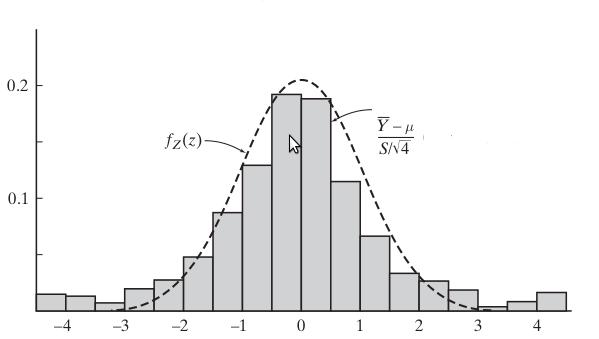
\includegraphics[height=5cm]{t1.png}


$t$ t Dagilimi (Student's t) ve Cauchy Dagilimi 

$X$, $v$ derece bagimsizlikta $t$ dagilimina sahiptir, ki bu $X \sim t_v$
diye yazilir eger 

$$ f(x) = 
\frac{ \Gamma(v+1)/2)} {\sqrt{v\pi}\Gamma(v/2)}
\bigg(1 + \frac{ x^2}{v}\bigg)^{-(v+1)/2}
 $$

$t$ dagilimi Normal dagilima benzer ama daha kuyrugu daha kalindir. Aslinda
Normal dagilimi $t$ dagiliminin $v = \infty$ oldugu hale tekabul
eder. Cauchy dagilimi da $t$'nin ozel bir halidir, $v = 1$ halidir. Bu
durumda yogunluk fonksiyonu

$$ f(x)  = \frac{ 1}{\pi(1+ x^2)} $$

Bu formul hakikaten bir yogunluk mudur? Kontrol icin entegralini alalim, 

$$ \int _{ -\infty}^{\infty} f(x) dx = 
\frac{ 1}{\pi} \int _{ -\infty}^{\infty} \frac{ dx}{1 + x^2} 
 $$

Cogunlukla entegre edilen yerde  ``1 arti ya da eksi bir seyin karesi''
turunde  bir ifade gorulurse, yerine gecirme (subsitution) islemi
trigonometrik  olarak  yapilir. 

$$  x = \tan \theta, \theta = \arctan x $$

$$ 1 + x^2 = 1 + \tan^2\theta = \sec^2\theta$$

$$ dx / d\theta = \sec^2\theta $$

O zaman 

$$ =
\frac{ 1}{\pi} \int _{ -\infty}^{\infty} \frac{ dx}{1 + x^2}   =
\frac{ 1}{\pi} \int _{ -\infty}^{\infty}  \frac{ 1}{\sec^2\theta}\sec^2\theta d\theta = 
\frac{ 1}{\pi} \int _{ -\infty}^{\infty}  1 \ d\theta = 
 $$

$$ = 
\frac{ 1}{\pi} \theta | _{ -\infty}^{\infty}   = 
\frac{ 1}{\pi} [\arctan(\infty) - \arctan(-\infty)]
 $$

$$ =
\frac{ 1}{\pi} [\frac{ \pi}{2} - (-\frac{ \pi}{2}) ] = 1
 $$


$\chi^2$ Dagilimi

$X$'in $p$ derece serbestlige sahip bir $\chi^2$ dagilima sahip ise $X \sim
\chi^2_p$ olarak gosterilir, yogunluk 

$$ f(x) = \frac{ 1}{\Gamma(p/2) 2^{p/2}} x^{(p/2) - 1} e^{-x/2 }, \ x > 0 $$

Eger $Z_1, .. , Z_p$ bagimsiz standart Normal rasgele degiskenler ise,
$\sum _{ i=1}^{p} Z_p \sim \chi^2_p$ esitligi dogrudur. 


\end{document}
